\section{Electromagnetic Induction}
\textbf{Electromagnetic induction} is the phenomenon where an e.m.f. is induced due to a changing magnetic field.

\subsection{Magnetic flux}
\begin{defn}{Magnetic flux $\Phi$}{}
Product of the component of the magnetic field density normal to the plane of the surface and the area of the
surface.
\begin{equation}
\Phi = B_{\perp}A = BA\cos\theta
\end{equation}
where $\theta$ is the angle between the normal of the plane and the magnetic field.
\end{defn}

Unit of magnetic flux is the weber (Wb). \textbf{Weber} is the flux of a uniform magnetic field $B$ of flux density $1\:\unit{T}$, through a plane surface of area $A$ of $1\:\unit{m^2}$, placed normally to the $B$ field.

\begin{figure}[H]
    \centering
    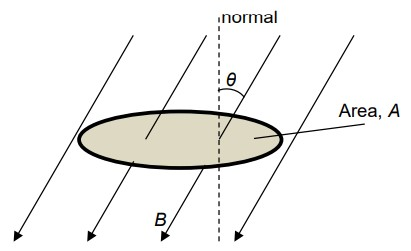
\includegraphics[width=8cm]{images/magnetic_flux.jpg}
\end{figure}

If area $A$ is bounded by a coil and the coil has $N$ turns, then the total magnetic flux passing through the coil (\textbf{magnetic flux linkage} through the coil) is
\begin{equation}
N\Phi = NBA\cos\theta
\end{equation}

From the equation, magnetic flux linkage through a coil depends on
\begin{itemize}
\item number of turns in coil $N$
\item magnitude of magnetic flux density $B$
\item surface area $A$
\item orientation of the coil $\theta$ with respect to the direction of $B$ ($\theta$ is the angle between the magnetic flux density and the normal of area of coil)
\end{itemize}

\begin{defn}{Magnetic flux linkage}{}
Product of magnetic flux passing through the coil and
number of turns on the coil.
\end{defn}
\pagebreak

\subsection{Laws of electromagnetic induction}
It was discovered experimentally that a changing magnetic field could induce an electric current in a circuit.

\begin{defn}{Faraday's law}{}
When the magnetic flux linkage with a circuit is changed, an induced e.m.f. is set up whose magnitude is directly proportional to rate of change of magnetic flux linkage.
\[ \varepsilon \propto \dv{(N\Phi)}{t} \]
\end{defn}

\begin{defn}{Lenz's law}{}
Induced e.m.f. (and hence current flow in a closed circuit)\footnote{A current is induced only if there is a complete circuit. An e.m.f. is always induced when there is a change in flux linkage.} is in a direction so as to produce effects which oppose the change that produces it.
\begin{equation}
\varepsilon = -\dv{(N\Phi)}{t} = -\dv{(NBA\cos\theta)}{t}
\end{equation}
\end{defn}

Lenz's Law is a consequence of the principle of conservation of energy.
\begin{itemize}
\item As the external agent brings the magnet towards the coil, by Lenz’s law, a current is induced in such a direction that the coil opposes, (i.e. repels) the approaching magnet.
\item Consequently, work has to be done by the external agent to overcome this opposition (the repulsive force).
\item It is this work done which is the source of the electrical energy.
\end{itemize}

\begin{tcolorbox}
\textbf{Fleming’s Right Hand rule}: determine direction of induced e.m.f. (and hence current in closed circuit).
\begin{itemize}
\item seCond finger represents Current
\item First finger represents magnetic Field
\item thumb represents force (or direction of motion)
\end{itemize}
\end{tcolorbox}

\subsubsection{Motional e.m.f. (Cutting of magnetic field)}
Motional e.m.f. is the e.m.f. induced in a conductor moving through a uniform magnetic field.

\begin{figure}[H]
    \centering
    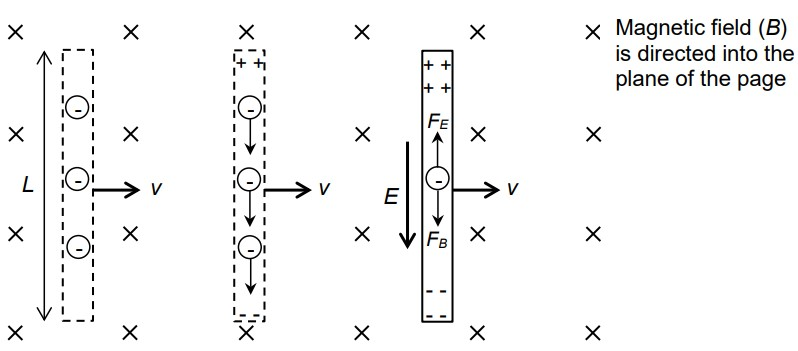
\includegraphics[width=12cm]{images/motional_emf.jpg}
\end{figure}

\begin{itemize}
\item When a conductor (wire) moves at a constant velocity in a uniform magnetic field, the moving conductor cuts magnetic field (or flux). An induced e.m.f. is generated when there is a cutting of flux. 
\item When the conductor is pushed to move to the right, free electrons in the conductor move to the right, so current flows to the left. Based on Fleming’s left-hand rule, each electron experiences downward magnetic force. 
\item Under the influence of this force, electrons move to the lower end of the conductor and accumulate there, leaving a net positive charge at the upper end. As a result of charge separation, electric field (directed downward) is produced inside the conductor. 
\item Charges accumulate at both ends until downward magnetic force is balanced by upward electric force.
\end{itemize}
\[ F_E = F_B \implies qE = qvB \implies E = vB \]

Since the electric field in the conductor is uniform, potential difference across the ends of conductor of length $L$ is given by $\Delta V=EL$ thus
\begin{equation}
\varepsilon = BLv
\end{equation}

Therefore an e.m.f. $\varepsilon$ is induced as long as the conductor continues to move through the uniform magnetic field. If the direction of the motion is reversed, polarity of induced e.m.f. is also reversed.

In summary, induced e.m.f. is also proportional to the rate of flux cutting.

For a moving conductor on a circuit with a resistance $R$ connected in series,
\[ \Delta V = BLv \implies \boxed{I=\frac{BLv}{R}} \]
\pagebreak

\subsection{Applications}
\subsubsection{Generator}
Electric generators take in energy by work and transfer it out by electrical transmission. 

\subsubsection{Eddy currents}
When a conductor is subjected to a changing magnetic flux, induced e.m.f. causes currents to flow. If the conductor is in the shape of a loop, induced current flows around the loop. However if the conductor is a solid plate, induced currents, known as \textbf{Eddy currents}, flow simultaneously along many different paths in swirls.

This can be demonstrated by allowing a flat copper or aluminium plate attached to the end of a rigid bar to swing back and forth through a magnetic field. As the plate enters the field, the plate cuts the magnetic field/flux. The changing magnetic flux induces an e.m.f. in the plate. The field in the plate is not uniform and the rate of cutting is not the same over the whole plate, so different e.m.f. are induced in different parts of plate, leading to eddy currents in the plate.

[figure]

As the swinging plate enters the field at position 1, the flux due to the external magnetic field into the page through the plate is increasing, hence by Lenz's law the induced eddy current must provide its own magnetic field out of the page. Direction of the induced current is thus anticlockwise. The opposite is true as the plate leaves the field at position 2, where the current is clockwise.

\paragraph{Applications}
set up a braking system which can rapidly change kinetic energy to other forms of energy. This can be taken a step further if a circuit can be built to channel the electrical energy from the kinetic energy back into the battery. This is what most hybrid cars do.

Stop rollercoasters, galvanometers, voltmeters and ammeters.

\paragraph{Drawbacks}
Eddy currents are dissipated as heating in the conductor (i.e. the conductor gets heated up).

Loss of energy in applications such as a transformer, as induced currents do work and raise the temperature of the iron core and cause energy loss.

Eddy currents can be reduced by eliminating paths for the current flow, for example, by cutting slits in the plate. These slits will prevent large eddy currents from occurring.
\pagebreak

\subsection*{Problems}

\pagebreak